\documentclass[a4wide,fontsize=12pt]{article}
\usepackage[utf8]{inputenc}
\usepackage{scrextend}
\usepackage{authblk}
%\usepackage[russian,english]{babel}
\usepackage[english]{babel}
\usepackage{amsmath}
\usepackage[left=2cm,right=2cm,
    top=2cm,bottom=2cm,bindingoffset=0cm]{geometry}
\usepackage{amsfonts}
\usepackage{bm}
\usepackage{graphicx}
\usepackage{hyperref}
\usepackage{comment}
\usepackage{tikz}
\usetikzlibrary{positioning}
\usetikzlibrary{patterns}
\usepackage{pgfplots}
\usepackage{multicol}
% \usepackage{filecontents}
\usepackage{animate}
\usepackage{graphics}

\usepackage{subcaption}
\usepackage{caption}

\usepackage{tikz}
\usetikzlibrary{decorations.pathreplacing}

\title{\textbf{Methods of visualisation for flows with internal waves attractors}}
\author[1,A]{D.A Ryazanov}
\author[2,B]{S.A. Elistratov}
\author[3,C]{I.N. Sibgatullin}
\author[4,A]{M.V.~Kraposhin}

\affil[A]{Ivannikov Institute for System Programming of the RAS}
\affil[B]{Lomonosov Moscow State University}
\affil[C]{Shirshov Institute of Oceanology of Russian Academy of Sciences}
\affil[ ]{}
\affil[1]{ORCID: 0000-0001-9568-7121}
\affil[2]{ORCID: 0000-0002-7006-6879}
\affil[3]{ORCID: 0000-0003-2265-3259}
\affil[4]{ORCID: 0000-0001-5730-2702}

%Ivannikov Institute for System Programming of the RAS, Lomonosov Moscow State University, Shirshov Institute of Oceanology of Russian Academy of Sciences.

\date{}

\begin{document}

\maketitle

\underline{\textbf{Abstract}}

Application of different approaches to visualize hydrodynamic fields of internal waves is closely connected with the possibility of extracting important numerical characteristics of the flows. In this paper we describe methods of visualisation, which were shown to be very effective for the illustration of the internal wave attractors both for laboratory experiments and numerical simulations. On the other hand, some novel approaches for description of the wave flows with accumulation of energy are discussed. Methods of vortices identification show interesting properties of the wave flows, and may give an alternative for the estimation of the width of wave beams. At the same time, the limitations of the applicability of the described methods strongly depend on the space and time resolution of the available data, which is especially important in the areas of the internal wave beam reflection.  

\textbf{Keywords:} CFD, internal waves, inertial waves, post-processing, wave attractor

\section{Introduction}

Internal waves are may be the most common types of waves in oceans, since even if the ocean surface seems to be calm, the deep-ocean waves \cite{1966MunkAbyssalRecipes,Munk1998} are always present\footnote{Gravity waves in the ocean's interior are as common as waves at the sea surface\,--\,perhaps even more so, for no one has ever reported an interior calm~\cite{2005Munk9IW}}. Oceanologists, biologists, ecologists, and technician have specific  interests in the study of internal waves. This phenomenon is partly responsible for the vertical mixing of the stratified fluids, the migration of living organisms, the redistribution of energy in the ocean, and the propagation of various kinds of impurities and pollution.

Despite a great diversity of experimental approaches for visualisation of weakly compressible flows \cite{znamenskaya2021methods388562176,2014SutherlandDuaxoisPeacockIWinLE}, the experiments are often bounded by the possibility to assess some interesting propriety at certain time location. Concerning the internal attractors and accompanying phenomena, remarkable advantages have been achieved since 199X. Besides the successful application of traditional approaches based on synthetic schlieren, particle image velocimetry (PIV) and laser-induced fluorescence (LIF) , some methods based on signal analysis, which traditionally were applied to electromagnetic fields, showed remarkable relevance for description of the internal or inertial wave dynamics. Meanwhile the time and space resolution of these methods is limited, and sometimes the laboratory data do not allow to reconstruct the hydrodynamic fields: 

Internal wave appear as a result of violation of stably stratified fluid. 
One of the major sources of perturbation, resulting in internal waves, is the tidal effect produced by the orbital motions of the Moon and the Sun. These global flows interact with the ocean bottom irregularities and generate internal waves. The very special feature of the internal waves is that in case of constant stratification the angle of the wave beams and the law of reflection are defined by the dispersion relation:
$$\frac{\omega}{N} = \sin(\theta),$$
where $\omega$ is the forcing frequency determined by external forcing on the fluid; 
$N$~-- buoyancy frequency.

% Пояснительная картинка с распространением
% Фокусировка внутренних волн

Due to these properties internal waves can be focused upon reflection from the oblique wall. As a consequence,  the internal wave wavelength is reduced upon reflection but its amplitude increases.

% Аттракторы внутренних волн
% картинка с резервуаром

The great interest is the result of the consecutive reflections. It can be obtained by the monochromatic excitation of the internal waves in the closed domain with the oblique boundaries, the simplest example of which is the rectangular trapezoid.

If the internal waves beams propagate in trapezoid tank, focusing occurs continuously and all the wave beams converge to closed trajectory. The simplest one is the rhomboid trajectory with four reflection points (Fig. \ref{fig:Domain}).

%  \flashleft
\begin{figure}[!Ht]
    % \centering
    %\flashleft
    \hspace{-1.8cm}
    \begin{minipage}[t]{0.45\textwidth}
        \begin{tikzpicture}[scale=1.5, z={(-.707,-.5)}]
            \draw (3.6,0,0) -- (0,0,0) -- (0,4,0)--(6,4,0)--(3.6,0,0);
            %\draw (3.6,0,0) -- (3.6,0,-1) -- (6,4,-1) -- (6,4,0) -- cycle;
            %\draw (6,4,0) -- (0,4,0) -- (0,4,-1) -- (6,4,-1);
            \node[anchor=south west,inner sep=0] at (0,0) {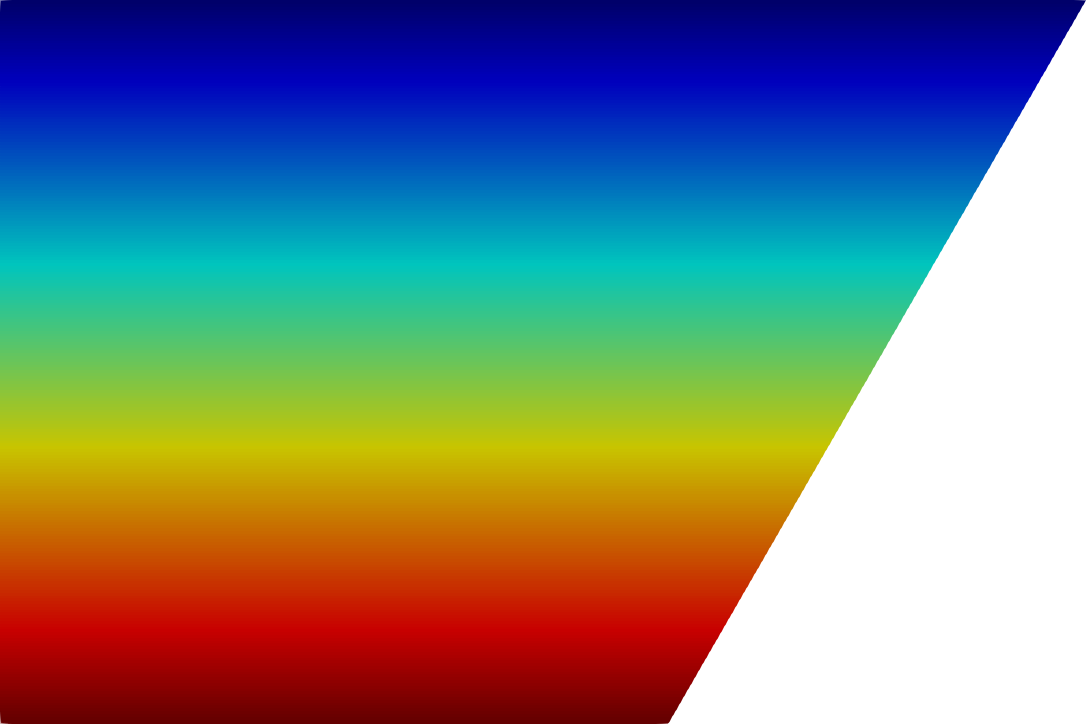
\includegraphics[width=1.15\textwidth]{Figs/Temp.png}};
            \draw (-0.5,2,0) node{};
            \draw (4.1,-.2,-1.5) node{};
            \draw [white] (3,3.8,0) node{$\rho_l = 1040$};
            \draw (1.8,2.1) node{$\rho_p = 1080$};
            \draw (3.1,2.1) node{$\rho_l = 1060$};
            \draw (2,0.2,0) node{$\rho_l = 1080$};
            \draw[<->] (-0.1,0) --node[above,rotate=90] {$H$} (-0.1,4);
            \draw[<->] (0,4.1,0) --node[above,] {$L_1$} (6,4.1,0);
            \draw[<->] (0,-0.1,0) --node[below,] {$L_2$} (3.7,-0.1,0);
            \draw [white, thick] (5.5,4) arc [start angle=180, end angle=240, radius=0.5cm]
        node [left] {$\alpha$};
            \draw[thick,->] (4.5,0.2,0) -- (5.5,0.2,0) node[anchor=north east]{$x$};
            \draw[thick,->] (4.5,0.2,0) -- (4.5,1+0.2,0) node[anchor=north west]{$z$};
            \draw[white,thick,->] (0,4.05,0) -- (1.5,2.8,0) ;
            \draw[thick,dotted] (0,2,0)--(4.8,2,0);
            \draw [white, thick] (0.0,3.5) arc [start angle=270, end angle=270+53, radius=0.5cm] node [below] {$\theta$}; 
        \end{tikzpicture}
    \subcaption{Initial distribution of density. $\rho_l$ -- density of liquid, $\rho_l$ -- density of particles, $\theta = \arcsin \frac{\omega}{N}$, where $\omega$ is frequency of wavemaker and $N$ is the buoyancy frequency.}
    \label{fig:domainup}
        \end{minipage}
% \end{figure}
~~~~
% \begin{figure}[b]
    \centering
        \begin{minipage}[t]{0.45\textwidth}
        \begin{tikzpicture}[scale=1.5]
            \draw [decorate,decoration={brace,amplitude=10pt},xshift=-4pt,yshift=0pt] (-0.2,0.0) -- (-0.2,4.1) node[rotate=90,above] [black,midway,xshift=-0,yshift=10] { Wavemaker};
            \node[anchor=south west,inner sep=0] at (0,0) {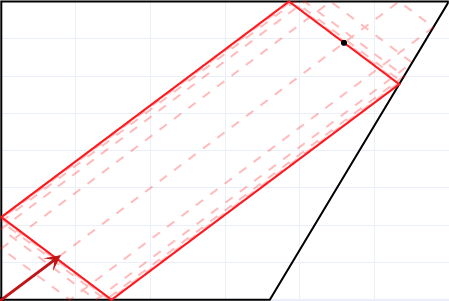
\includegraphics[width=1.15\textwidth]{Figs/Dom.png}};
%     \node[anchor=south west,inner sep=0] at (0,0) {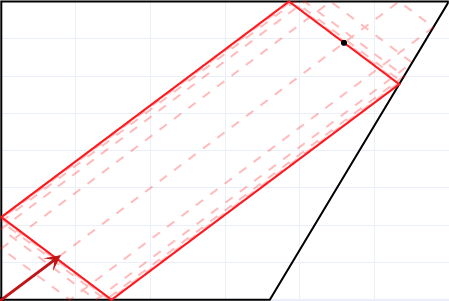
\includegraphics[width=0.5265\textwidth]{Figs/Dom.png}};
            \draw[thick,<->] (-0.1,0) --node[above,rotate=90]{$H$} (-0.1,4.1);
            \draw[thick,<->] (0,-0.1) --node[below          ]{$L_2$} (3.8,-0.1);
            \draw[thick,<->] (0,4.2) --node[above          ]{$L_1$} (6.2,4.2);
            \draw [black, thick] (5.75,4.1) arc [start angle=180, end angle=270, radius=0.25cm];
        \end{tikzpicture}
    \subcaption{Principal scheme of the vessel}
    \label{fig:Domain}
    \end{minipage}
    \caption{Scheme of computational domain for 2D attractor of internal waves. Initial destribution of density (a), and predicted with linear theory shape of attractor (b).}
\end{figure}

%\begin{figure}[!ht]
%    \centering
%        \begin{tikzpicture}[scale=1.5, z={(-.707,-.5)}]
%            \draw (0,4-0,0) -- (6,4-0,0) -- (4,4-4,0)--(0,4-4,0) --cycle;
%            \draw (0,4-0,0)     -- (6,4-0,0)   -- (4,4-4,0)   -- (0,4-4,0)    -- cycle;
%            \draw[style = dashed,red] (2.7,4-4,0)   -- (0,4-1.8,0) -- (2.2,4-0,0) -- (4.97,4-2.1,0)-- cycle;
%            \draw[<->] (-0.1,4-0) --node[above,rotate=90] {$H$} (-0.1,4-4);
%            \draw[<->] (0,4+0.1,0) --node[above,] {$L_2$ } (6,4+0.1,0);
%            \draw[<->] (0,4-4.1,0) --node[below,] {$L_1$ } (4,4-4.1,0);
%            \draw[thick,->] (4.95,4-4,0) -- (5.95,4-4,0) node[anchor=north east]{$x$};
%            \draw[thick,->] (4.95,4-4,0) -- (4.95,4-3,0) node[anchor=north west]{$z$};
%            \draw[thick,->] (5.5,4-2,0) -- (5.5,4-3,0) node[anchor=west]{$\vec{g}$};
%        \end{tikzpicture}
%    \caption{Scratch of the domain and attraction area}
%    \label{fig:dominleft}
%\end{figure}

For the first time the phenomenon of wave attractors was described by Leo Maas \cite{Maas1995} who studied the convergence of wave beams while considering different geometries.

First attempts of numerical study~\cite{2008GrisouardStaquetPairaud} of internal wave attractors successfully reproduced qualitatively the 2D structure of internal wave attractors in trapezoidal domains, though quantitatively the velocity amplitude was too high  as compared with the experiment. 3D numerical simulations~\cite{2016BrouzetSibgatullinScolanErmanyukDauxois,2016BrouzetErmanyukJoubaudSibgatullinDauxois} resolved this problem through estimation of viscosity and boundary layers effects.

In this paper we apply the before-mentioned methods for numerical results, and discuss the other methods, which are difficult to assess in the experiments.

\section{Problem statement and solution methods}

For the stratified fluid dynamic simulation quasihydrodynamic equations were used \cite{ElizarBook}: 

 \begin{equation}
     \nabla \cdot \left (\vec U - \vec W \right ) = 0,
     \label{eq:cont}
 \end{equation}
 \begin{equation}
     \frac{\partial \vec U}{\partial t}  + \nabla \cdot \left ( (\vec U - \vec W)\otimes \vec U  \right )
     -
     \nabla \cdot \nu \left ( \nabla \vec U + (\nabla \vec U)^T \right ) - \nabla \cdot \left  (   \vec U \otimes \vec W \right ) 
      = - \frac{1}{\rho_m} \nabla \hat p + \vec F,
      \label{eq:mom}
 \end{equation}
     
 \begin{equation}
     \frac{\partial s}{\partial t} + \nabla \cdot \left ( (\vec U - \vec W)s \right )
     - \nabla \cdot \frac{\nu}{Sc} \left ( \nabla s \right )=0.
     \label{eq:tr}
 \end{equation}


Additional velocity:  $$\vec W = \tau \left ( \vec U \cdot \nabla \vec U + \frac{1}{\rho_m} \nabla \hat p - \vec F  \right ),$$\\

reduced pressure $\hat p = p - p_0$; restorative force: $\vec{F}=\beta \vec{g} \hat s$, where $\hat s = s(x, y, z, t) - s(x, y, z, 0).$

Geometrically the computational domain is the rectangular trapeze, on the left wall of which a wavemaker is situated. The letter one makes oscillations. 

Velocity boundary conditions on wavemaker depends on problem being solved.

Boundary conditions on static walls:

\begin{equation}\label{eq:qhd_walls}
        \vec{U} = 0, \,\,\, \frac{\partial \tilde p}{ \partial \vec{n}} = \rho_0 \vec n \cdot \left ( -\vec U_b \cdot \nabla \vec U + \vec F \right), \,\,\, \frac{\partial s}{ \partial \vec{n}} = 0.
\end{equation}

The initial conditions for a passive scalar are chosen so that the buoyancy frequency is equal to 1

\begin{equation}
    N(z) = \sqrt{- \frac{g}{\rho_m}\cdot\frac{d \rho(z)}{dz}} = 1,
\end{equation}

where $\rho(z) = \rho_m(1+\beta s)$  and $\beta$ -- coefficient of salinity contraction. 



Equations \ref{eq:cont}--\ref{eq:tr} solve by finite volume method and open source code OpenFOAM v2012 with QHDFoam solver \cite{QGDFOam}

\section{Post-processing and data analysis}

All data was collected using native openFoam functionObjects and processed by python-scripts. Fields was visualised by open-source, multi-platform data analysis and visualization application paraview \cite{paraview}. Scratches and schemes 

\subsection{2D statement}

As the calculation results, it is expected that internal waves will concentrate in the zone of attraction (fig.~\ref{fig:Domain}). In this case $H = 0.4 \; m$, $L_1=0.6 \; m$, $L_2 = 0.39 \; m$.

As boundary conditions on wavemaker:

\begin{equation}
    U_x = A\cdot cos\left(\frac{\pi \cdot z}{H}\right)\cdot \omega \cdot  sin(\omega_0 t),
    \label{eq:wmc}
\end{equation}
where $A = 0.003 \; m$, $\omega = 0.63 \; s^{-1}$.

For the further representation we will use herebelow wavemaker frequency $f_0=\tfrac{\omega_0}{2\pi}$ and corresponding period $T_0=f_0^{-1}$. 
Dynamic of velocity fluids field over time can be spit in two smooth parts.

Part of attractor formation (Fig. \ref{fig:LamAttr}). Internal waves reflect from slope wall and aim to attractor with increasing own aplitude.

Part of attractor destruction (Fig. \ref{fig:turbAttr}). Gradually amplitude grows so much that the waves begin to overturn and generate child waves.

\begin{figure}
\centering
    \begin{minipage}[t]{0.45\textwidth}
        \centering
            %\animategraphics[autoplay,loop,scale=0.21]{10}{Figs/2DAttractorForm/300x200a03w0623.0}{180}{200}
            \subcaption[fir]{Sedimentation from $t=0\,s$ to $t=80\,s$}
        \label{fig:LamAttr}
    \end{minipage}
    \begin{minipage}[t]{0.45\textwidth}
        \centering
            %\animategraphics[autoplay,loop,scale=0.21]{10}{Figs/2DAttractorDest/300x200a03w0623.7}{160}{199}
            \subcaption[sec]{Redistribution from $t=3590 \,s$ to $t=3600$}
        \label{fig:turbAttr}
    \end{minipage}
    \caption{Horizontal component of velocity field with internal wave focusing}
\end{figure}


Visualisation of velocity field was provided by paraview software \cite{paraview}. The pictures \ref{fig:LamAttr} and \ref{fig:turbAttr} show horizontal component.

As the one of main method of flow motions analysis time-frequency diagram which shows dynamic of spectrum is considered (Fig. \ref{fig:tfd11}-\ref{fig:tfdX}). In fact it is the Fourier-transform made with a sliding window in dependence on window's position. Hence, vertical slices of the diagram are spectra at neighbourhood of time moment $t$, so one can trace the evolution of the spectrum. At the beginning of motion fluid has one clear frequency, but then attractor destruction leads to the generation of secondary waves and contamination of the spectrum, that appears as a noising background on the diagram. 

% \begin{figure}
% \begin{multicols}{2}
%     \centering
%     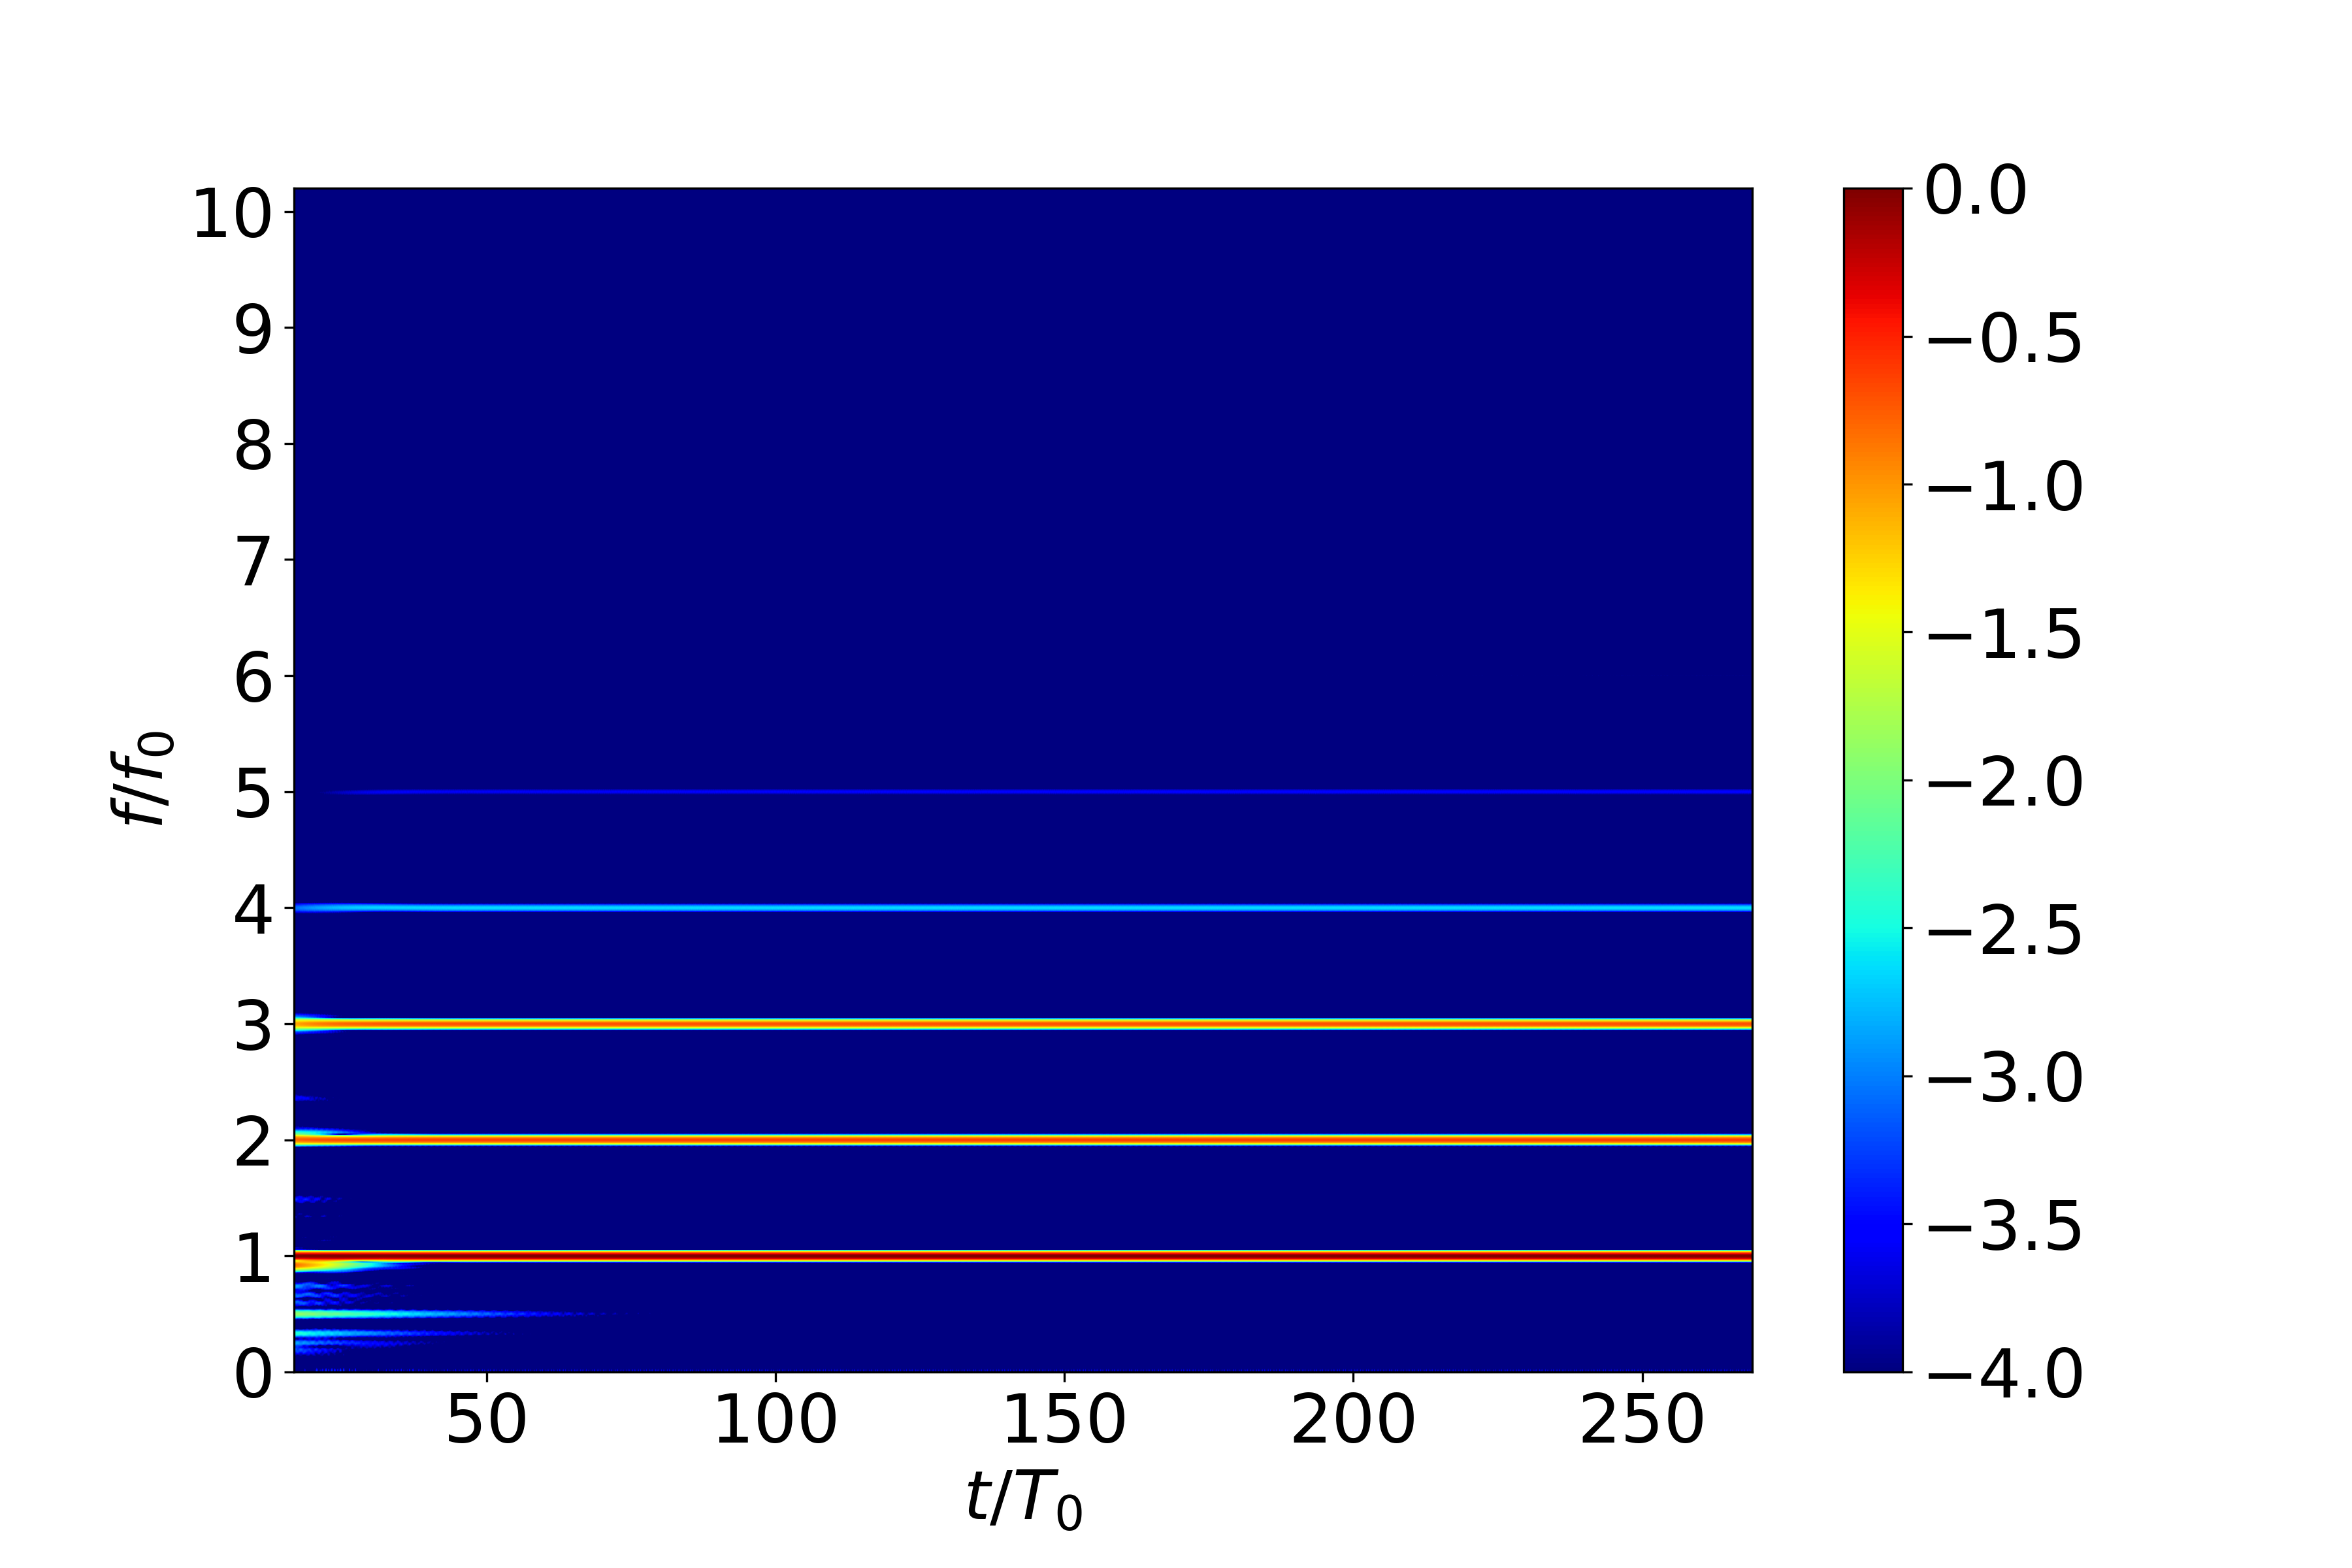
\includegraphics[width=0.55\textwidth]{Figs/TFBG14.png}
%     \caption{Time-frequency diagram of superharmonics presence ($a=1.4\;mm$)}
%     \label{fig:tfd11}
%     \hfill
%      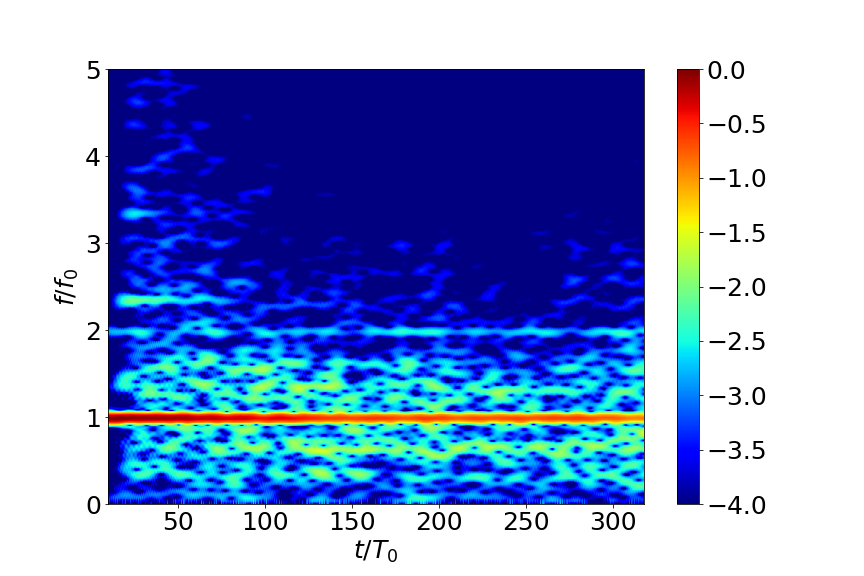
\includegraphics[width=0.55\textwidth]{Figs/TFD_pos34693_nperseg400_to0T.png}
%     \caption{Time-frequency diagram of attractor destruction ($a=3.0\;mm$)}
%     \label{fig:tfdX}
% \end{multicols}
% \end{figure}


\begin{figure}
\centering
    \begin{minipage}[t]{0.45\textwidth}
        \centering
        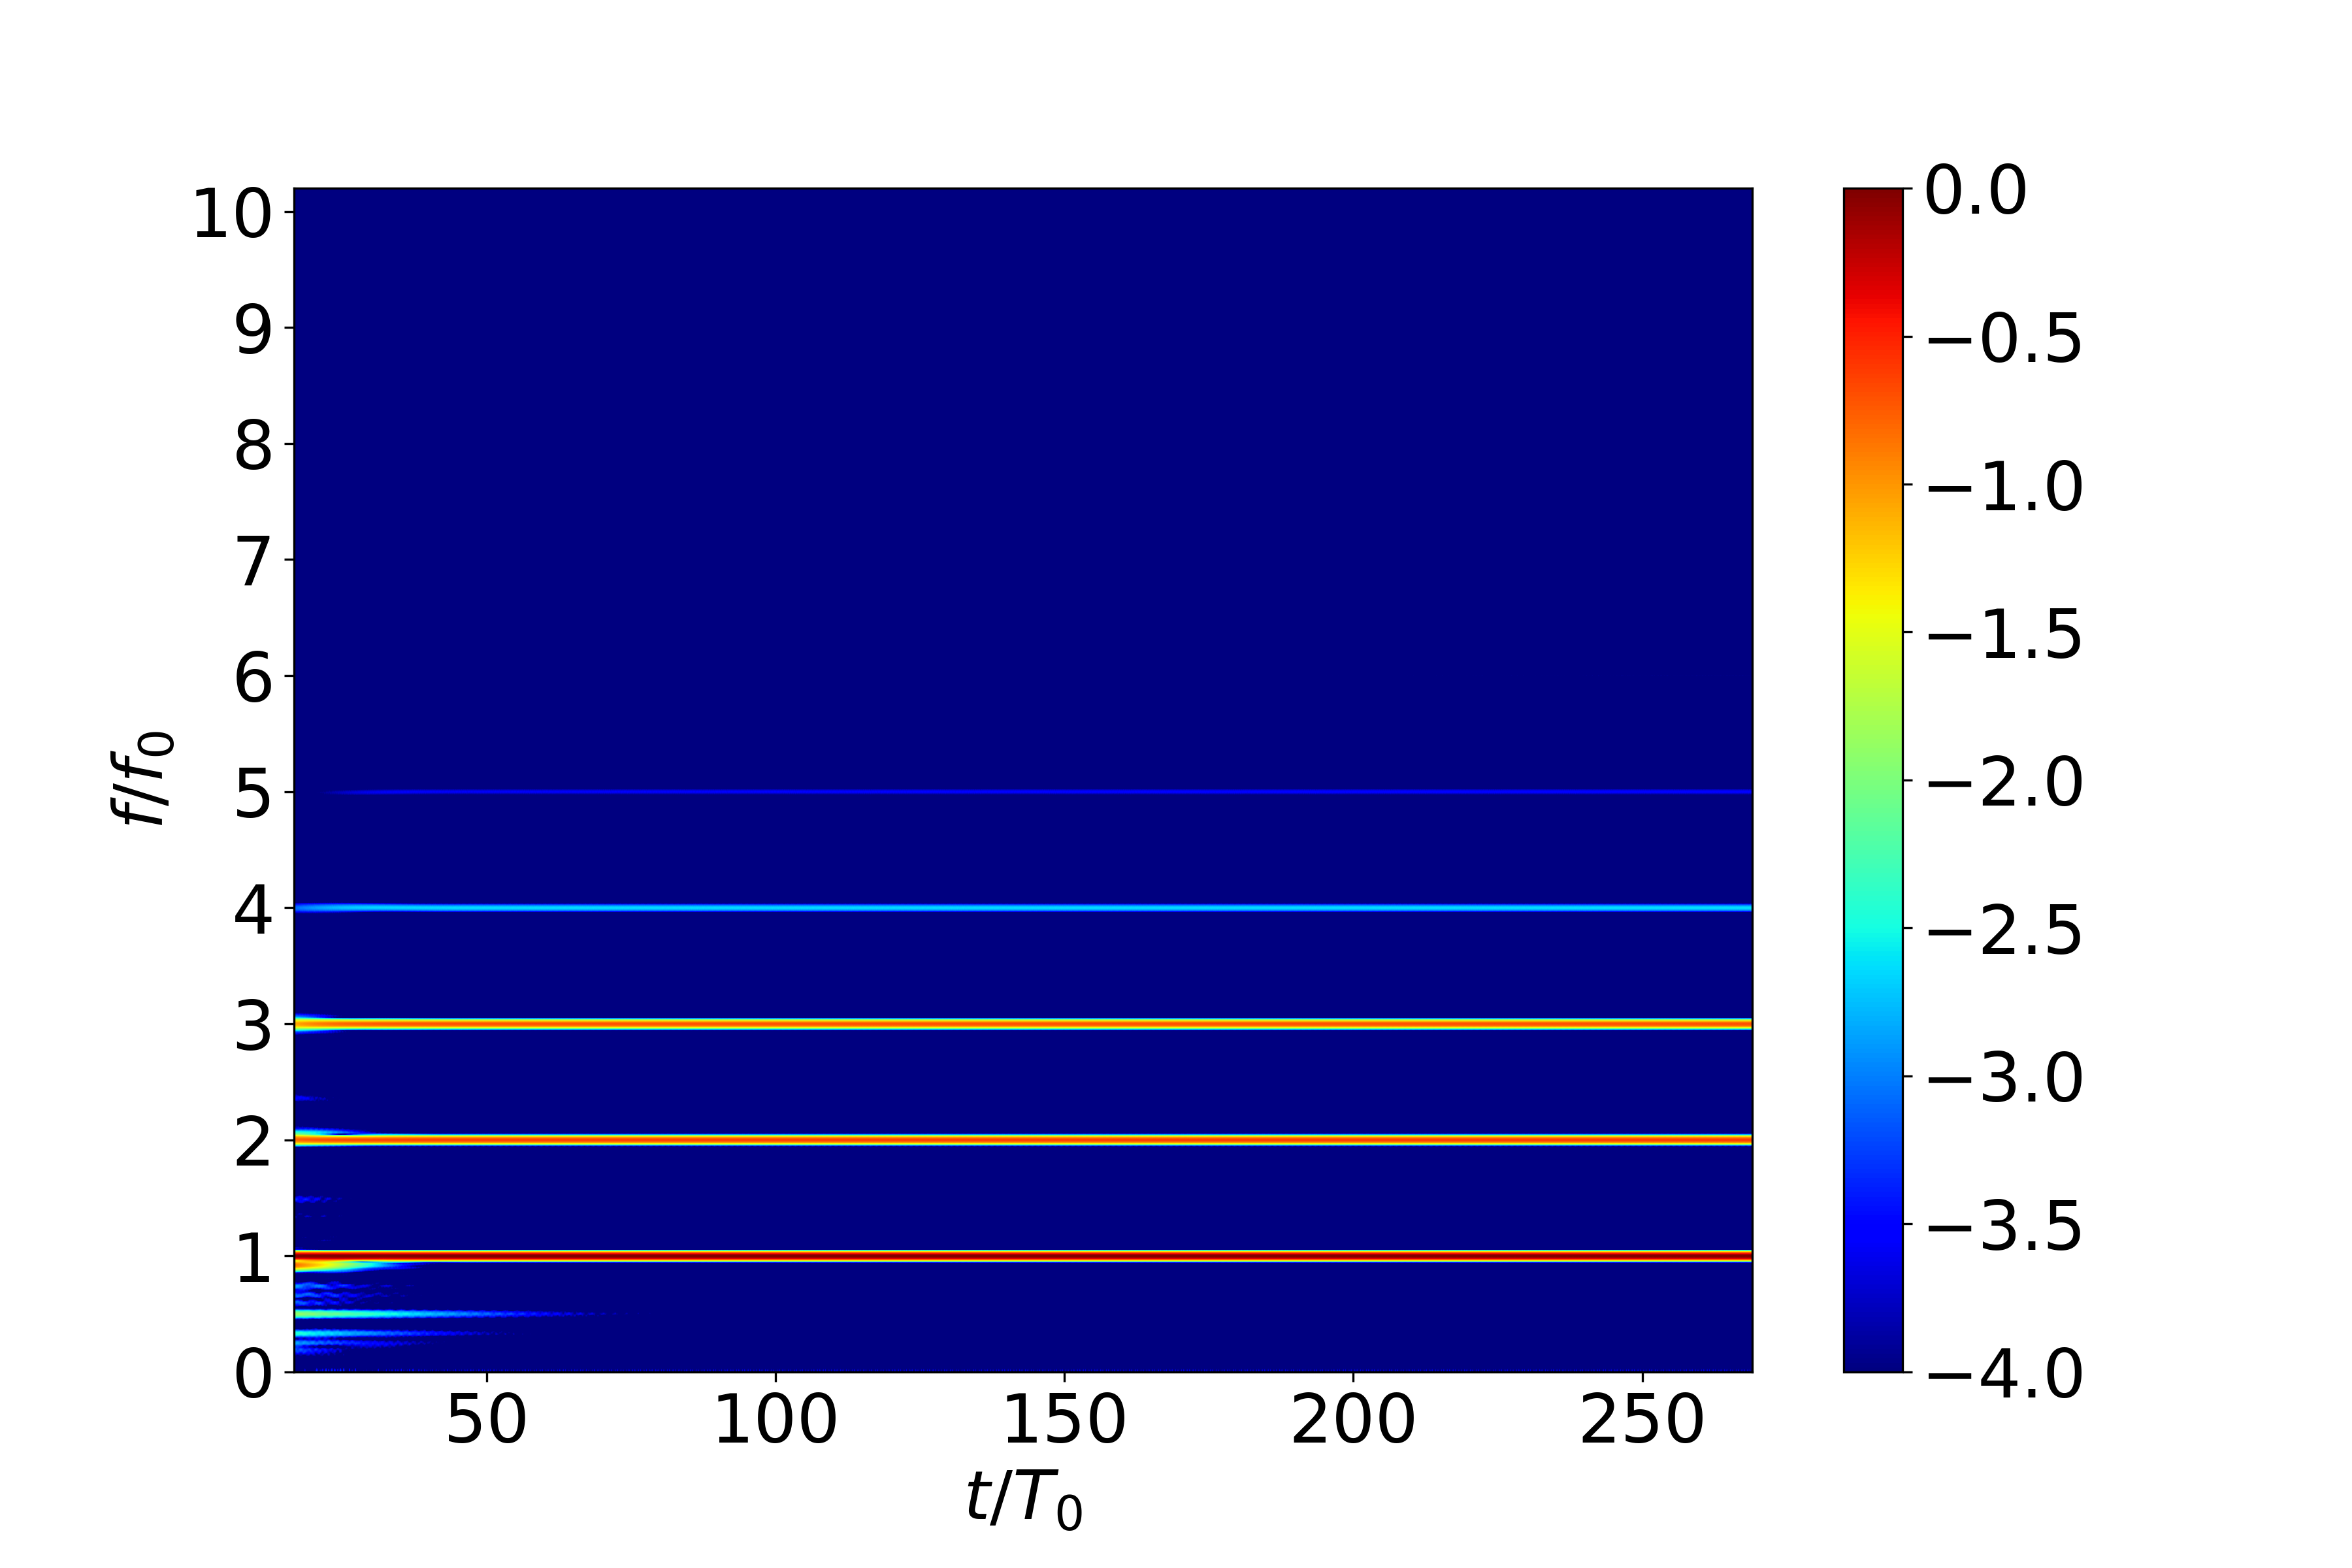
\includegraphics[width=1.15\textwidth]{Figs/TFBG14.png}
        \subcaption[fir]{Time-frequency diagram of superharmonics presence ($a=1.4\;mm$)}
        \label{fig:tfd11}
    \end{minipage}
    \begin{minipage}[t]{0.45\textwidth}
        \centering
        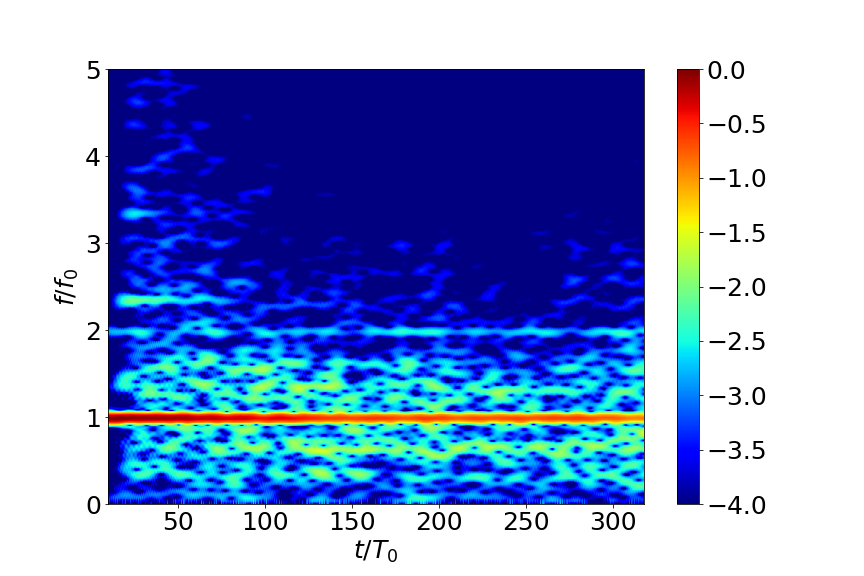
\includegraphics[width=1.15\textwidth]{Figs/TFD_pos34693_nperseg400_to0T.png}
        \subcaption[sec]{Time-frequency diagram of attractor destruction ($a=3.0\;mm$)}
        \label{fig:tfdX}
    \end{minipage}
    \caption{Time-frequency diagrams}
\end{figure}


Figures \ref{fig:tfd11}-\ref{fig:tfdX} illustrate dependence of time-frequency diagrams on the forcing amplitude (colorbar shows the ratio of $\lg\left(\frac{TF}{\text{max} (TF)}\right)$ in order to normalize the maximum to 0).  If the amplitude is not high enough, spectrum almost doesn't evolve and has discrete peaks; with its increase spectrum becomes continuous and fluctuates with the time, which indicates the complete transition to the turbulent regime.

\subsection{Sedimentation}

One of the important problems is a simulation of low inertial particles sedimentation. Distribution of density in  the reservoir is linear from $1040\;\frac{kg}{m^3}$ to $1080\;\frac{kg}{m^3}$, at the center of the reservoir puts spherical particles with density $\rho_p = 1080;\frac{kg}{m^3}$ and diameter $d=0.001 \; m$.  Number of particles is 301 over horizontal middle line (Fig. \ref{fig:domainup}). Particles are carried away by the flow, but do not affect it and one another.

The simulation is of interest for two reasons: sedimentation process before particles touch the bottom and distribution process after sedimentation. Numerical experiment was carried out in two different statements for wavemaker conditions (\ref{eq:wmc}) with $A_1=0.05e^{-2}\;m$ -- regime of stable attractor without destruction and child waves and $A_2=0.003\;m$ turbulent attractor of internal waves from previous subsection. 

\begin{figure}
\centering
    \begin{minipage}[t]{0.45\textwidth}
        \centering
    %\animategraphics[autoplay,loop,scale=0.12]{10}{Figs/2DSedTurbBegin/AnimationRho1080C0r01mmslip.0}{001}{159}
    \animategraphics[autoplay,loop,scale=0.12]{10}{Figs/2DSedTurbBegin/AnimationRho1080C0r01mmslip.0}{001}{002}
        \subcaption[fir]{Sedimentation from $t=0\,s$ to $t=80\,s$}
        \label{fig:turbSed2Da}
    \end{minipage}
    \begin{minipage}[t]{0.45\textwidth}
        \centering
    %\animategraphics[autoplay,loop,scale=0.125]{10}{Figs/2DSedTurbEnd/AnimationRho1080C0r01mmslip.7}{013}{052}
    \animategraphics[autoplay,loop,scale=0.125]{10}{Figs/2DSedTurbEnd/AnimationRho1080C0r01mmslip.7}{013}{014}
        \subcaption[sec]{Redistribution from $t=3590 \,s$ to $t=3600$}
        \label{fig:turbSed2Db}
    \end{minipage}
    \caption{Sedimentation in reservoir with turbulent regime of internal waves attractor}
\end{figure}

Numerical experiment shown that particles slow fall and redistribute (Fig. \ref{fig:turbSed2Da}). Fallen particles concentrate about two attraction center at the bottom (Fig. \ref{fig:turbSed2Db}) after a long time of simulation ($1000-2000\ s$).

Changing of experemint condition for amplitude of wamaket to $A_1$ leads to the fact that attractor do not redistribute particles after sedimentation. Also, the attractor is too weak to significantly influence to process of sedimentation.

\begin{figure}
\centering
    \begin{minipage}[t]{0.45\textwidth}
        \centering
        
        %\animategraphics[autoplay,loop,scale=0.2]{10}{Figs/AttrctorSlipLaminarSediment/SlipLam.0}{000}{159}
        \animategraphics[autoplay,loop,scale=0.2]{10}{Figs/AttrctorSlipLaminarSediment/SlipLam.0}{000}{001}
        \subcaption[fir]{Sedimentation from $t=0\,s$ to $t=80\,s$}
        \label{fig:turbSed2Da}
    \end{minipage}
    \begin{minipage}[t]{0.45\textwidth}
        \centering
        %\animategraphics[autoplay,loop,scale=0.2]{10}{Figs/AttrctorSlipLaminarMid/SlipLam.07}{40}{79}
        \animategraphics[autoplay,loop,scale=0.2]{10}{Figs/AttrctorSlipLaminarMid/SlipLam.07}{40}{41}
        \subcaption[sec]{Redistribution from $t=3590 \,s$ to $t=3600$}
        \label{fig:turbSed2Db}
    \end{minipage}
    \caption{Sedimentation in reservoir with turbulent regime of internal waves attractor}
\end{figure}

\subsection{3D local wavemaker}


        \begin{figure}
        \centering
          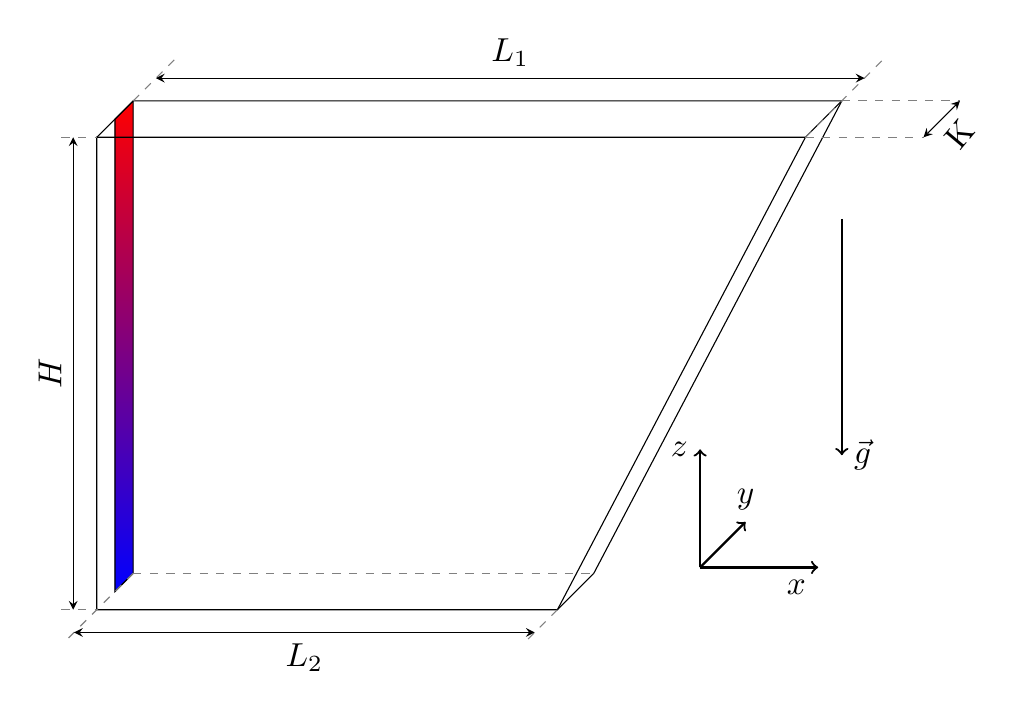
\begin{tikzpicture}[scale=1.5, every node/.style={scale=1.2}]
            \filldraw[top color=red, bottom color=blue] (0,0,0)--(0,0,0.4)--(0,4,0.4)--(0,4,0)--cycle;
            
            \draw (0,4,0.0) -- (6,4,0.0)-- (3.9,0,0.0);
            \draw (3.9,0,0.8) -- (0,0,0.8) -- (0,4,0.8) -- (6,4,0.8) -- cycle;
             
            \draw (0,4,0) -- (0,4,0.8);
            
            \draw (3.9,0,0) -- (3.9,0,0.8);
            \draw (6,4,0) -- (6,4,0.8);
    
            % \draw[style=dashed, color=gray] (6,0,-3) -- (0,0,-3) -- (0,4,-3);
            \draw[style=dashed, color=gray] (0,0,0) -- (0,0,1.5);
            \draw[style=dashed, color=gray] (3.9,0,0.8) -- (3.9,0,1.5);
            
            \draw[style=dashed, color=gray] (0,4,0) -- (0,4,-1.);
            \draw[style=dashed, color=gray] (6,4,0.8) -- (6,4,-1.);
            
            \draw[stealth-stealth] (0,4,-0.5)--node[above]{$L_1$}(6,4,-0.5);
            
            \draw[stealth-stealth] (0,0,1.3)--node[below]{$L_2$}(3.9,0,1.3);
            
            \draw[style=dashed, color=gray] (0,0,0) -- (3.9,0,0);
            
            \draw[style=dashed, color=gray] (6,4,0.8) -- (7,4,0.8);
            \draw[style=dashed, color=gray] (6,4,0.0) -- (7,4,0.0);
            \draw[stealth-stealth] (7,4,0.8)--node[below,rotate=50]{K}(7,4,0.0);
            % \draw (-0.5,2,0) node{};
            % \draw (4.1,-.2,-3.5) node{};
            % \draw (3.5,5,0) node{};
            \draw[stealth-stealth] (-0.2,0,0.8) --node[above,rotate=90] {$H$} (-0.2,4,0.8);
            \draw[style=dashed, color=gray] (-0.3,0,0.8) -- (0.0,0,0.8);
            \draw[style=dashed, color=gray] (-0.3,4,0.8) -- (0.0,4,0.8);
            
            
            % \draw[<->] (0,4.1,-3) --node[above,] {$L_1 = 0.369$ m} (4,4.1,-3);
            % \draw[<->] (6.05,-0.05,0) --node[below,rotate=37] {$W = 0.3$ m} (6.05,-0.05,-3);
            % \draw[<->] (0,-0.1,0) --node[below,] {$L_2 = 0.6$ m} (6,-0.1,0);
            % \draw [black, thick] (3.75,4) arc [start angle=180, end angle=300, radius=0.25cm]
            % node [anchor = south west] {$120^\circ$};
            \draw[thick,->] (4.8,0.05,0) -- (5.8,0.05,0) node[anchor=north east]{$x$};
            \draw[thick,->] (4.8,0.05,0) -- (4.8,1.05,0) node[anchor=east]{$z$};
            \draw[thick,->] (4.8,0.05,0) -- (4.8,0.05,-1) node[anchor=south]{$y$};
            \draw[thick,->] (6,3,0) -- (6,1,0) node[anchor=west]{$\vec{g}$};
          \end{tikzpicture}
          
        \caption{Illustration of 3D domain with local wavemaker in numerical experiment $H=0.4\ m$, $L_1 = 0.6\ m$, $L_2 = 0.39\ m$, $K=0.08 \ m$.}
        \label{fig:3DLocSctarch}
        \end{figure}

\begin{figure}[!Ht]
\centering
    \begin{minipage}{0.45\textwidth}
        \centering
            %\animategraphics[autoplay,loop,scale=0.11]{10}{Figs/3DPartTurbAttr6/3dTurbPartA6.00}{01}{40}
            \subcaption[f]{Stable phase of internal waves attractor for local wavemaker from $t=150\,s$ to $t=170\,s$}
        \label{fig:3DTurbBegin}
    \end{minipage}
    \begin{minipage}{0.45\textwidth}
        \centering
            %\animategraphics[autoplay,loop,scale=0.11]{10}{Figs/3DPartTurbAttr6/3dTurbPartA6.02}{59}{99}
            \subcaption[s]{Turbulisation of internal waves attrctor with local wavemaker from $t=280\,s$ to $t=300\,s$}
        \label{fig:3DTurbEnd}
    \end{minipage}
    \caption{Life cycle of internal waves attractor from stability to chaos. Color visualisation of velocity horizontal component. Flare in reservoir is a interprocessors interfaces painted in salinity colorbar where $1$ is a blue and $2$ is a red. Wall with wave maker has a different color scale: from $-0.001\,m/s$ to $0.001\,m/s$.}
    \label{fig:3DLocTurbRes}
\end{figure}



\subsection{Vortices visualisation}

Vortices visualisation is a new way to visualize turbulent motions structure. For this purpose we use different methods.

The simplest attempt is to consider vorticity \cite{vortex}, fig.~\ref{fig:vorticity}: $$\omega=|\textrm{rot}\,\vec{v}|$$
It is quick and simple method that however can yield false-positive identification. For instance, Couette flow will be identified as homogeneous vortex since its curl is constant over the domain.

Another method is so-called $\Delta$-method \cite{vortex}. Let us consider eigenvalue problem for velocity gradient tensor $A=\nabla\otimes  \vec v$:

% \begin{equation}
%  A:= \nabla\otimes  \vec v =
% \begin{pmatrix}
%  \frac{\partial v_x}{\partial x}  & \frac{\partial v_x}{\partial y} \\ \frac{\partial v_y}{\partial x} & \frac{\partial v_y}{\partial y} 
% \end{pmatrix}
% \end{equation}

\begin{equation}
  \text{det} \,( A -\lambda \mathbb E)=0
\end{equation}  

In 3D we have the following characteristic equation: $$\lambda^3+P\lambda^2+Q\lambda+R,$$ \noindent which discriminant is $D=-108\left( \frac{Q^2}{4} +\frac{P^3}{27}\right)$. 


Let $$\Delta=\left(\frac{Q}{2}\right)^2 +\left(\frac{P}{3}\right)^3$$

$ \Delta > 0  \Leftrightarrow  D < 0$ means the presence of two complex-conjugated roots, i.e. current tubes is spiral-like shaped.

The problem arises in 2-dimensional problem, where the equation has less order:
$$\lambda^2+P\lambda+Q=0,$$

discriminant $D=P^2-4Q$. Thus in 2D we will consider $-D\equiv 4Q-P^2$ as $\Delta$ (fig.~\ref{fig:Delta}).

This method requires more computational resources than vorticity. It can be improved using $Q$-method \cite{vortex}\cite{Hussain}. Let's define:

\begin{equation}
 S=\frac{1}{2}\left(A +A\,^T \right) ,\quad \Omega=\frac{1}{2} \left( A - A\,^T\right) 
  \label{NSdim}
\end{equation}
Then
\begin{equation}
  Q=\frac{1}{2} \left( ||\Omega||^2_F-||S||^2_F \right) 
  \label{eqn:Q}
 \end{equation}
For the more courtesy we remind that norm in (\ref{eqn:Q}) is understood in sense of Frobenius norm, i.e. $||A||^2_F=\sum \limits_{i=1}^n \sum \limits_{j=1}^n a_{ij}^2$, where $n$ is problem dimention.

The vortex regions are those with $Q>0$. It is harder condition then that for the $\Delta$, so $Q$-identified vortex regions a priori contain in $\Delta$-identified ones (fig.~\ref{fig:Q}).

For the fourth method let's calculate eigenvalues of $A$. For the vortex presence it's necessary for two complex-conjugation values to exist. Their imaginary parts $\pm\lambda_{ci}$ that can be considered as the identification method itself \cite{vortex}, fig.~\ref{fig:Lci}.

If we consider eigenvalues of $S^2+\Omega^2$~matrix, we obtain $\lambda_2$-method. They cannot be complex, so for the vortex two negative ones are implied. Let's sort them in descending order and consider the second one as a criterion\cite{vortex,Hussain}. For the visibility we will display it with the opposite sign (hence 'tis negative), fig.~\ref{fig:L2}.

The most modern method is Luitex-method \cite{vortex}.

Let $\vec r \longleftrightarrow \lambda_r$~-- eigenvector corresponding to real eigenvalue $\lambda_r, ||\vec r||=1$. Then Luitex-vector is introduced as that with the direction of $\vec r$ and value
 $$R=(\vec \omega,\vec r)-\sqrt{(\vec \omega,\vec r)^2-4\lambda_{ci}^2},$$\noindent where $\vec \omega$ is vorticity. Wherein it's supposed that $(\vec \omega,\vec r)>0$.
 
 In 2-dimensional problem Luitex-vector must be re-defined. Obviously, vorticity is orthogonal to the domain plane as well as $\vec r$. Hence we consider only value
 
 $$R=|\omega|- \sqrt{\omega^2-4\lambda_{ci}^2},$$\noindent where $\omega=\frac{\partial v_y}{\partial v_x}-\frac{\partial v_x}{\partial v_y}$~-- two-dimensional vorticity (fig.~\ref{fig:Liu}).

\begin{figure}
\begin{multicols}{2}
    \centering
    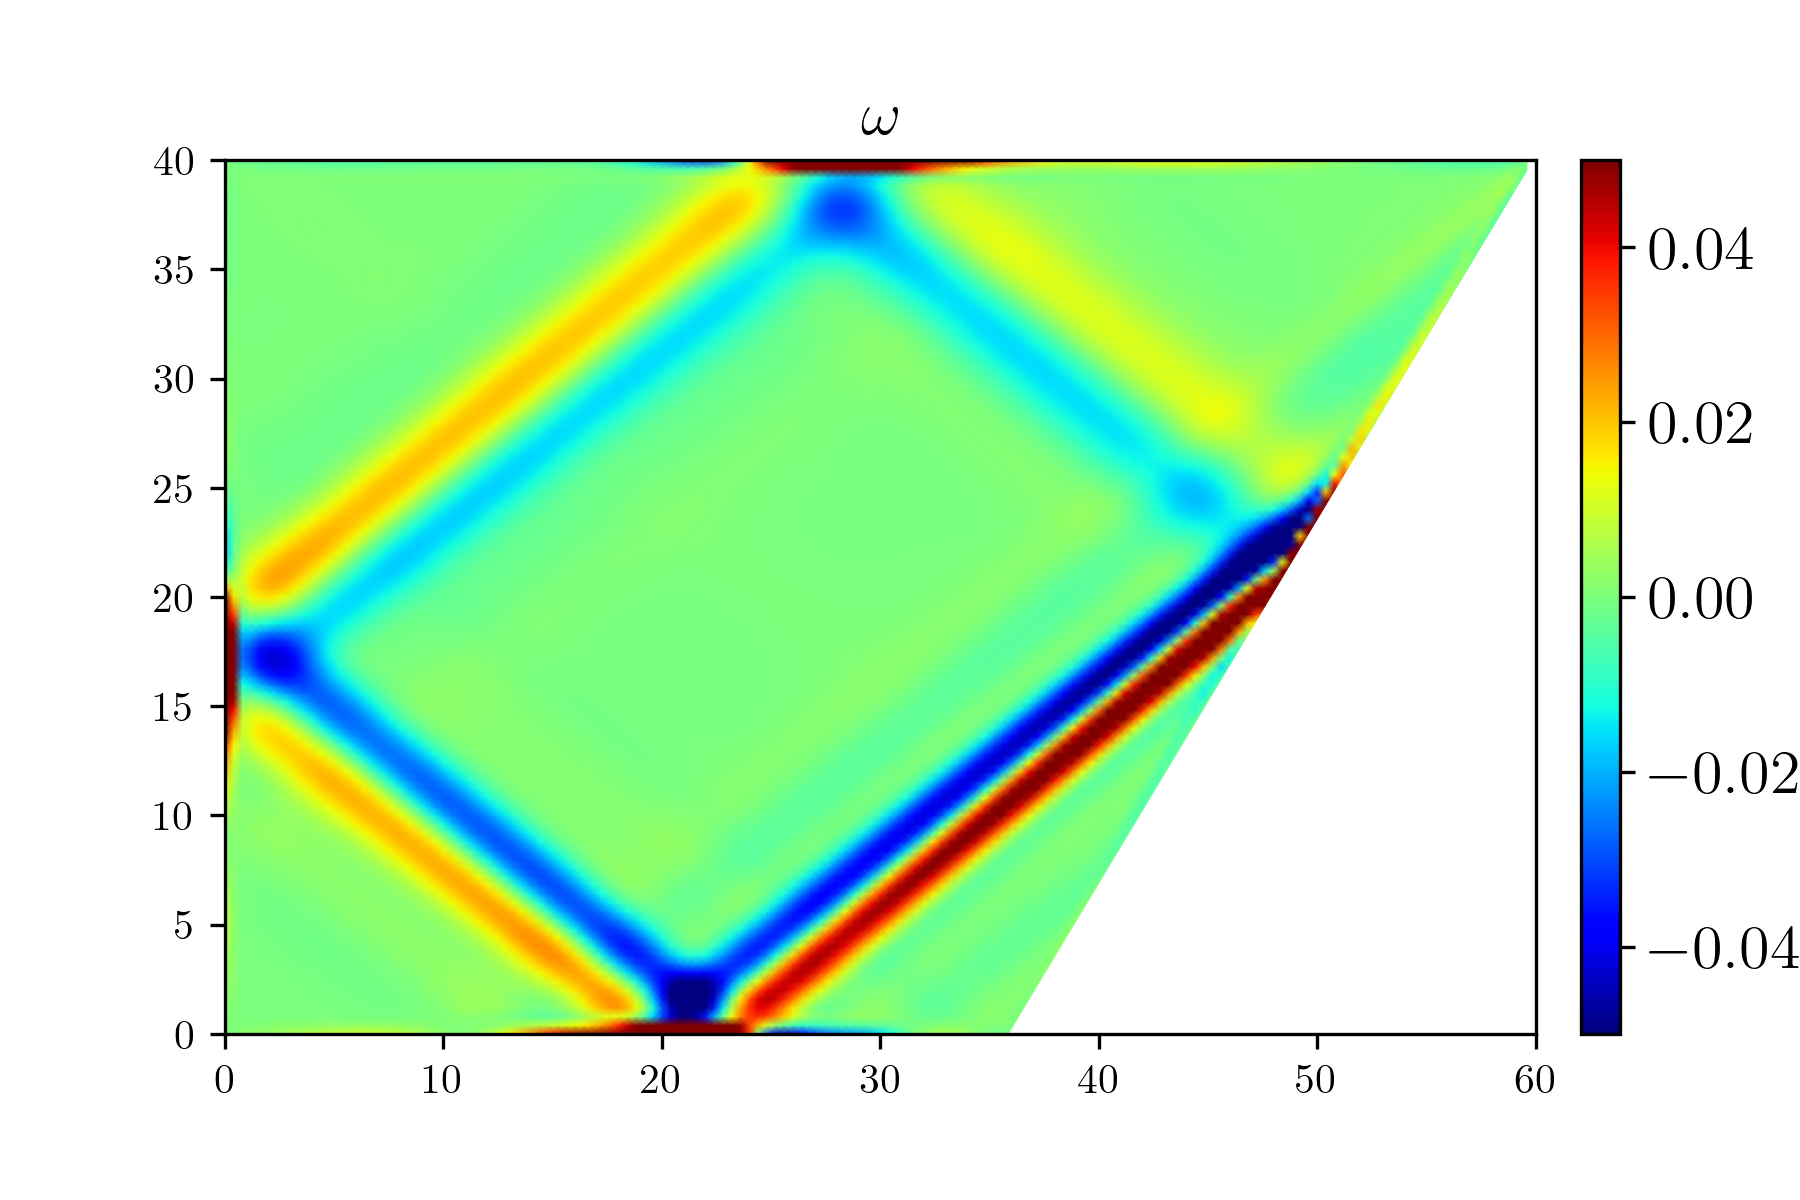
\includegraphics[width=0.5\textwidth]{Figs/VortexRot.png}
    \caption{vorticity}
    \label{fig:vorticity}
    \hfill
    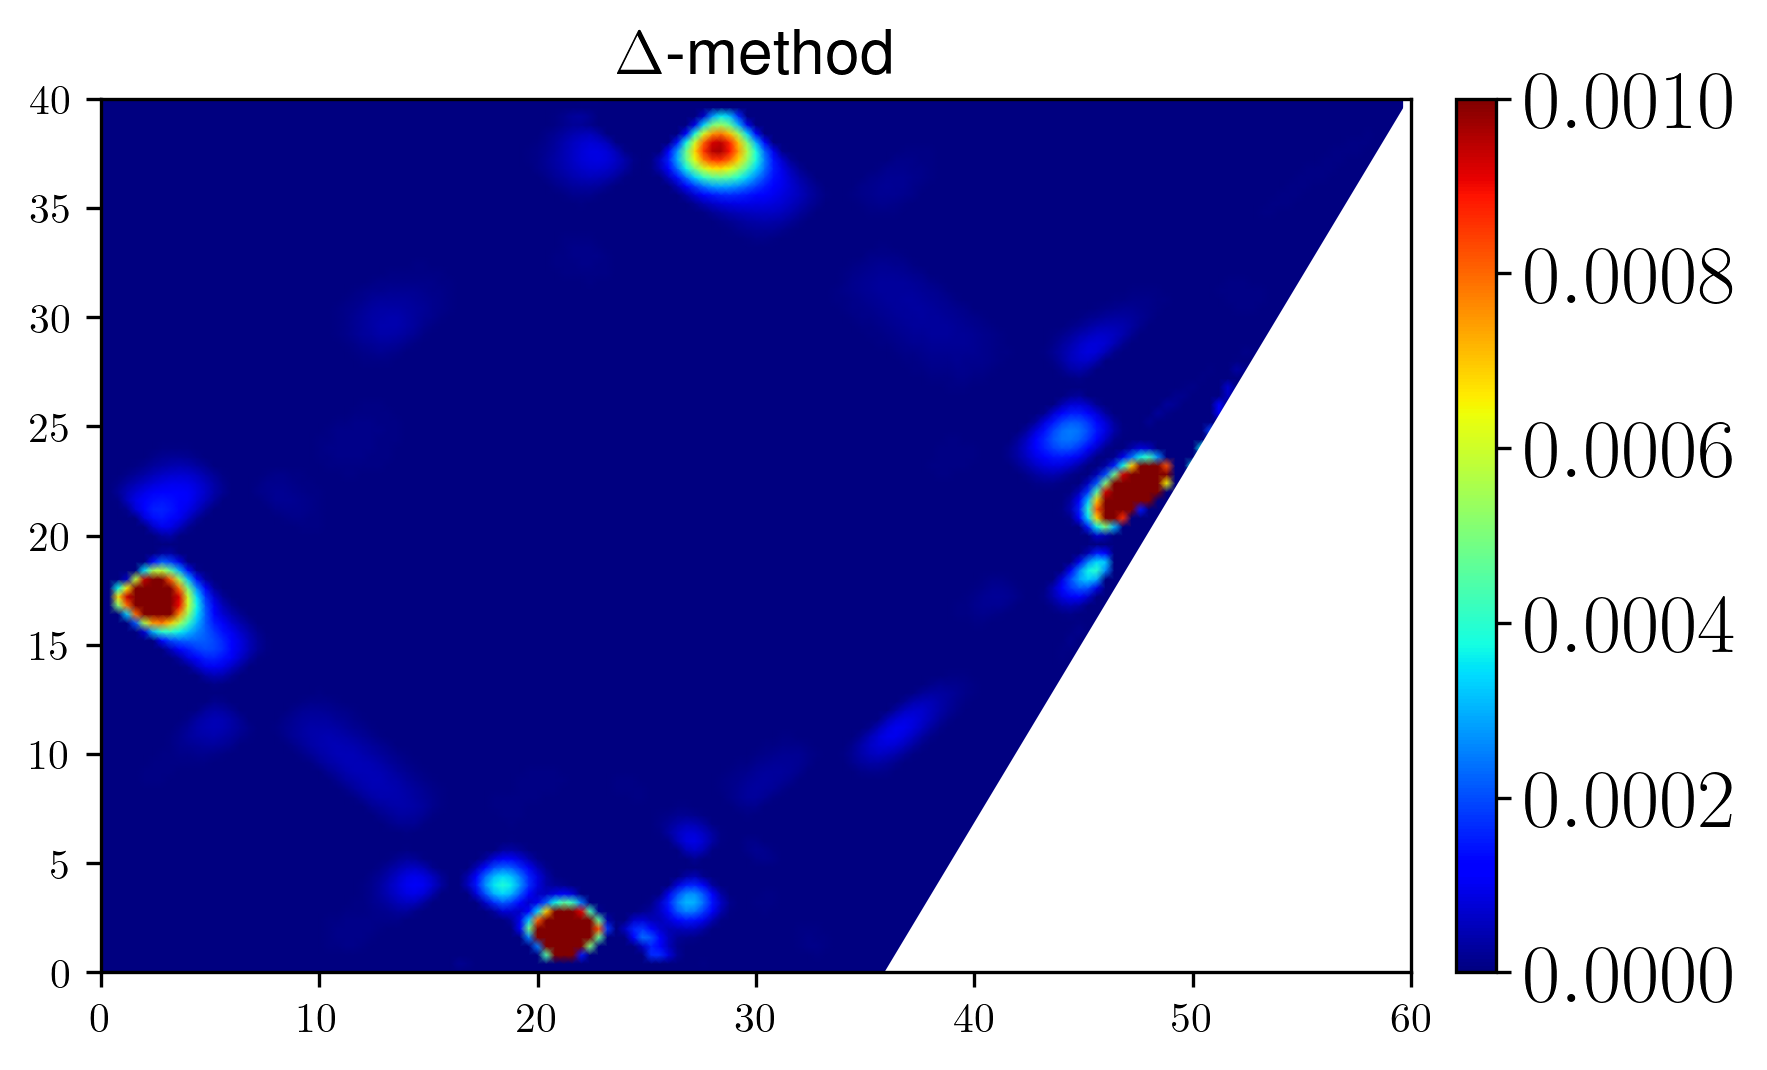
\includegraphics[width=0.5\textwidth]{Figs/VortexDelta.png}
    \caption{$\Delta$-method}
    \label{fig:Delta}
\end{multicols}
\end{figure}

\begin{figure}
\begin{multicols}{2}
    \centering
    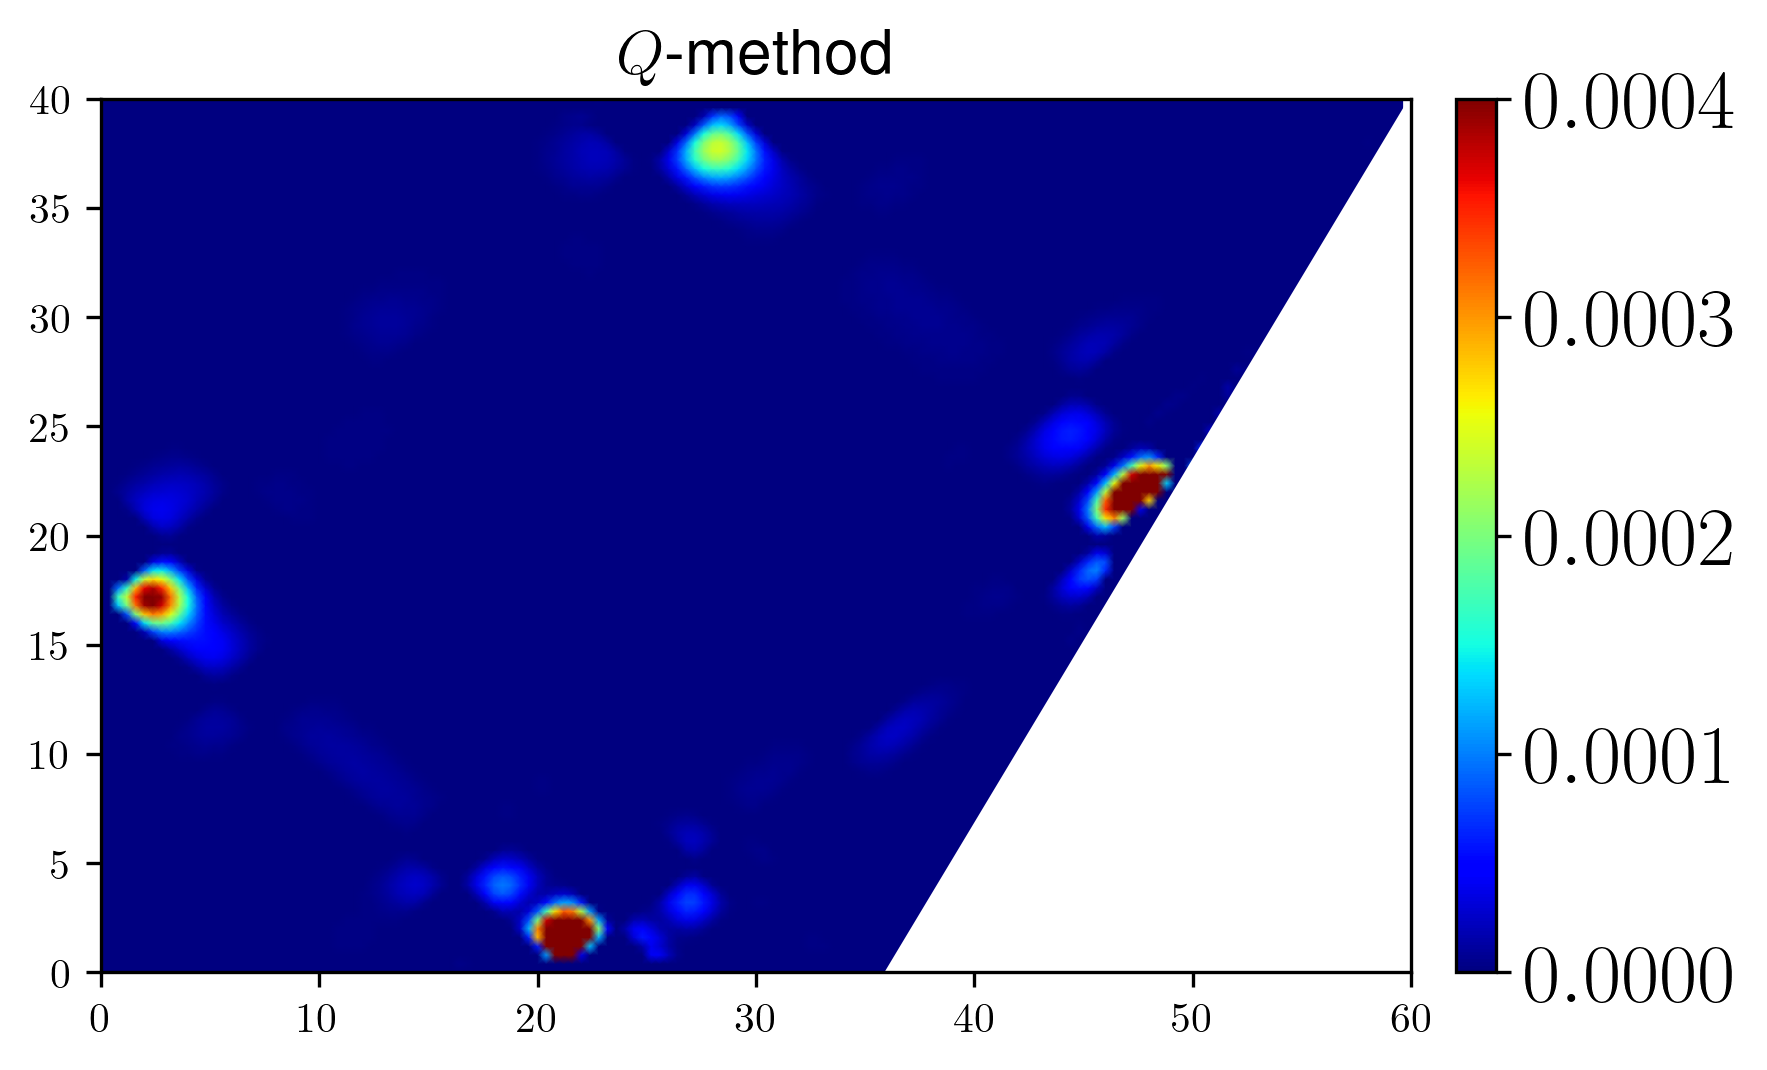
\includegraphics[width=0.5\textwidth]{Figs/VortexQ.png}
    \caption{$Q$-method}
    \label{fig:Q}
    \hfill
    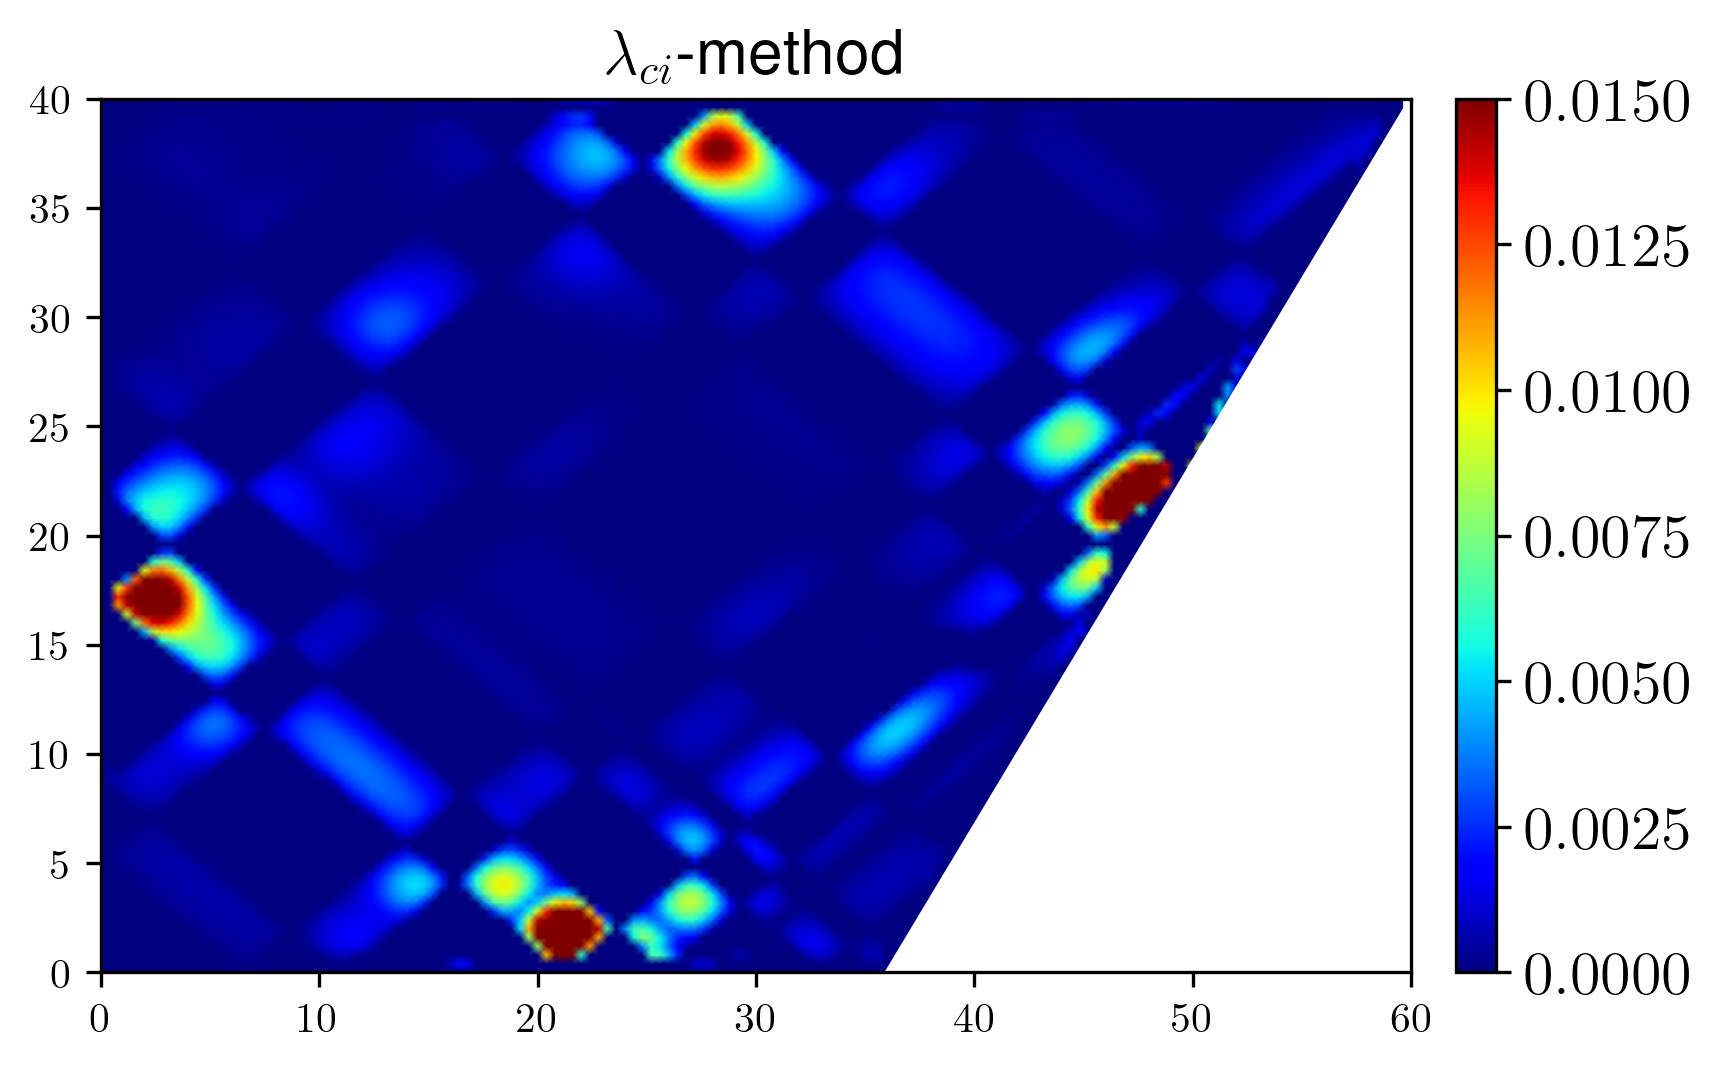
\includegraphics[width=0.5\textwidth]{Figs/VortexLambdaCi.png}
    \caption{$\lambda_{ci}$-method}
    \label{fig:Lci}
    \end{multicols}
\end{figure}

\begin{figure}
\begin{multicols}{2}
    \centering
    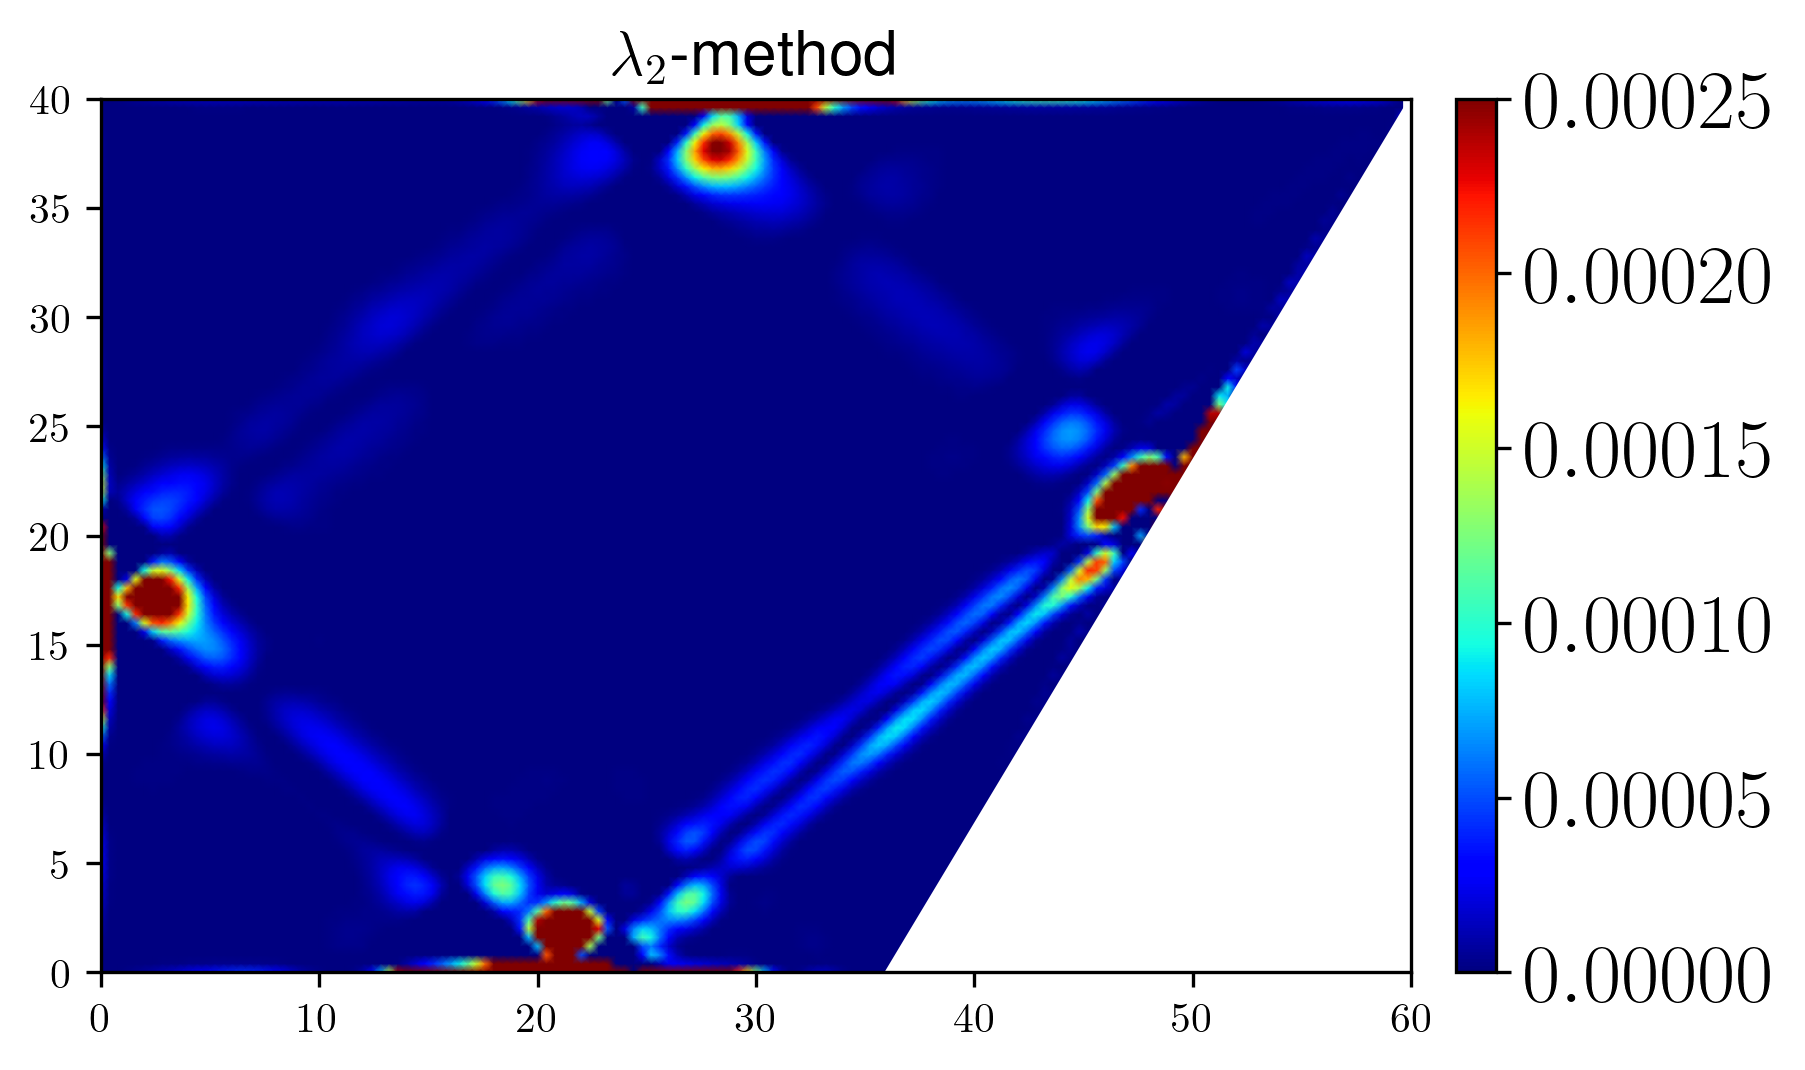
\includegraphics[width=0.5\textwidth]{Figs/VortexLambda2.png}
    \caption{$\lambda_2$-method}
    \label{fig:L2}
    \hfill
    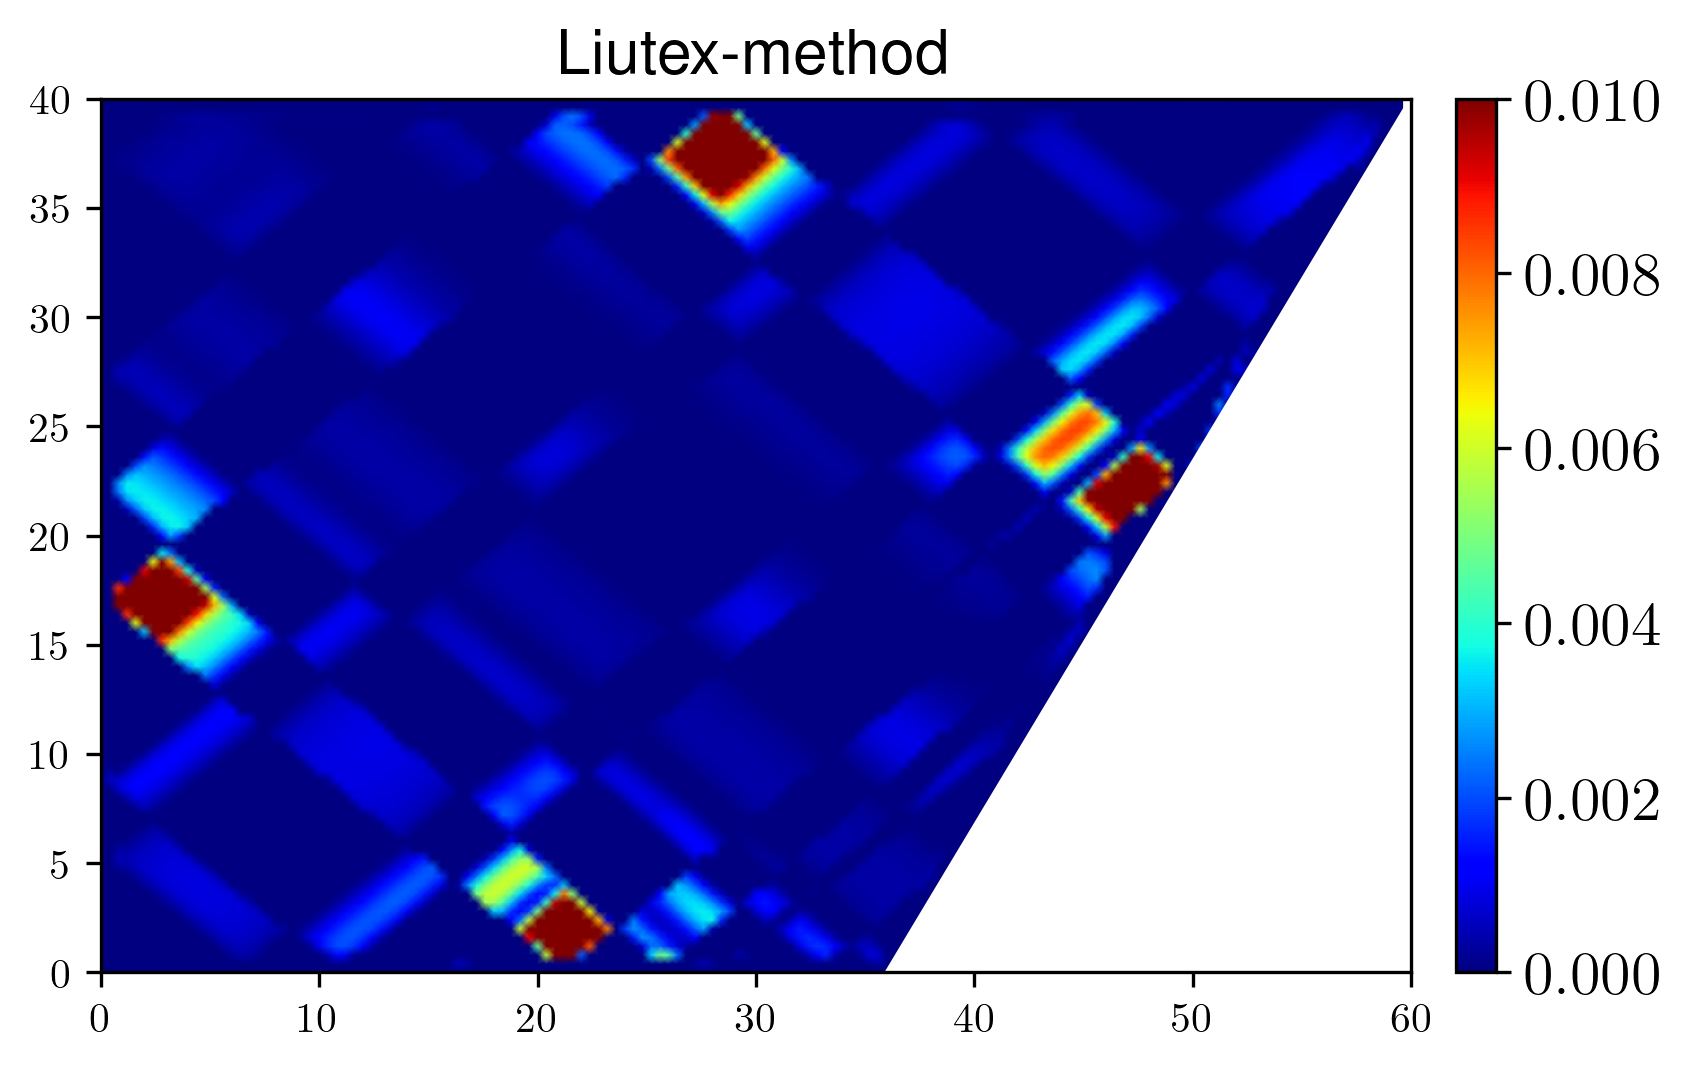
\includegraphics[width=0.5\textwidth]{Figs/VortexLui.png}
    \caption{Liutex-method}
    \label{fig:Liu}
    \end{multicols}
\end{figure}

Howbeit mentioned hereabove methods are aimed to visualize vortex regions, they can be sucsessfully applied for the attractor detection, at least at small enough amplitudes.

\section{Conclusions}

Visualization cannot be spread on bread.

\section{Acknowledgments}



The work will done with the support of Russian Scientific Fund, grant RSF~19-11-00169.
Authors thank T.G. Elizarova.

\bibliographystyle{ugost2008}
\bibliography{rpz,internalwaves}

\end{document}
